\chapter{Einleitung}
Dieses Dokument dient der genaueren Beschreibung und Dokumentation des Entwurfs zum Visualisierungstool \gls{programname}, dessen Hauptaufgabe die Darstellung des Netzwerkverkehrs eines \gls{profinet}-Systems ist. Des Weiteren wird der im IDS \gls{snort} eingebaute \gls{praeprozessor} \gls{sppname} und die genaue Funktionsweise der \gls{ipc} zu \gls{programname} genau erläutert.\newline
\newline
Das Design von \gls{programname} baut auf dem klassischen \gls{mvc} auf und erweitert diesen Entwurf zu einem \gls{mvp} mit zusätzlicher Funktionalität.

//hier MVC von Präsentation und ähnliches Bild zum aktuellen Entwurf einfügen//
 
\begin{figure}[H]
  \centering
  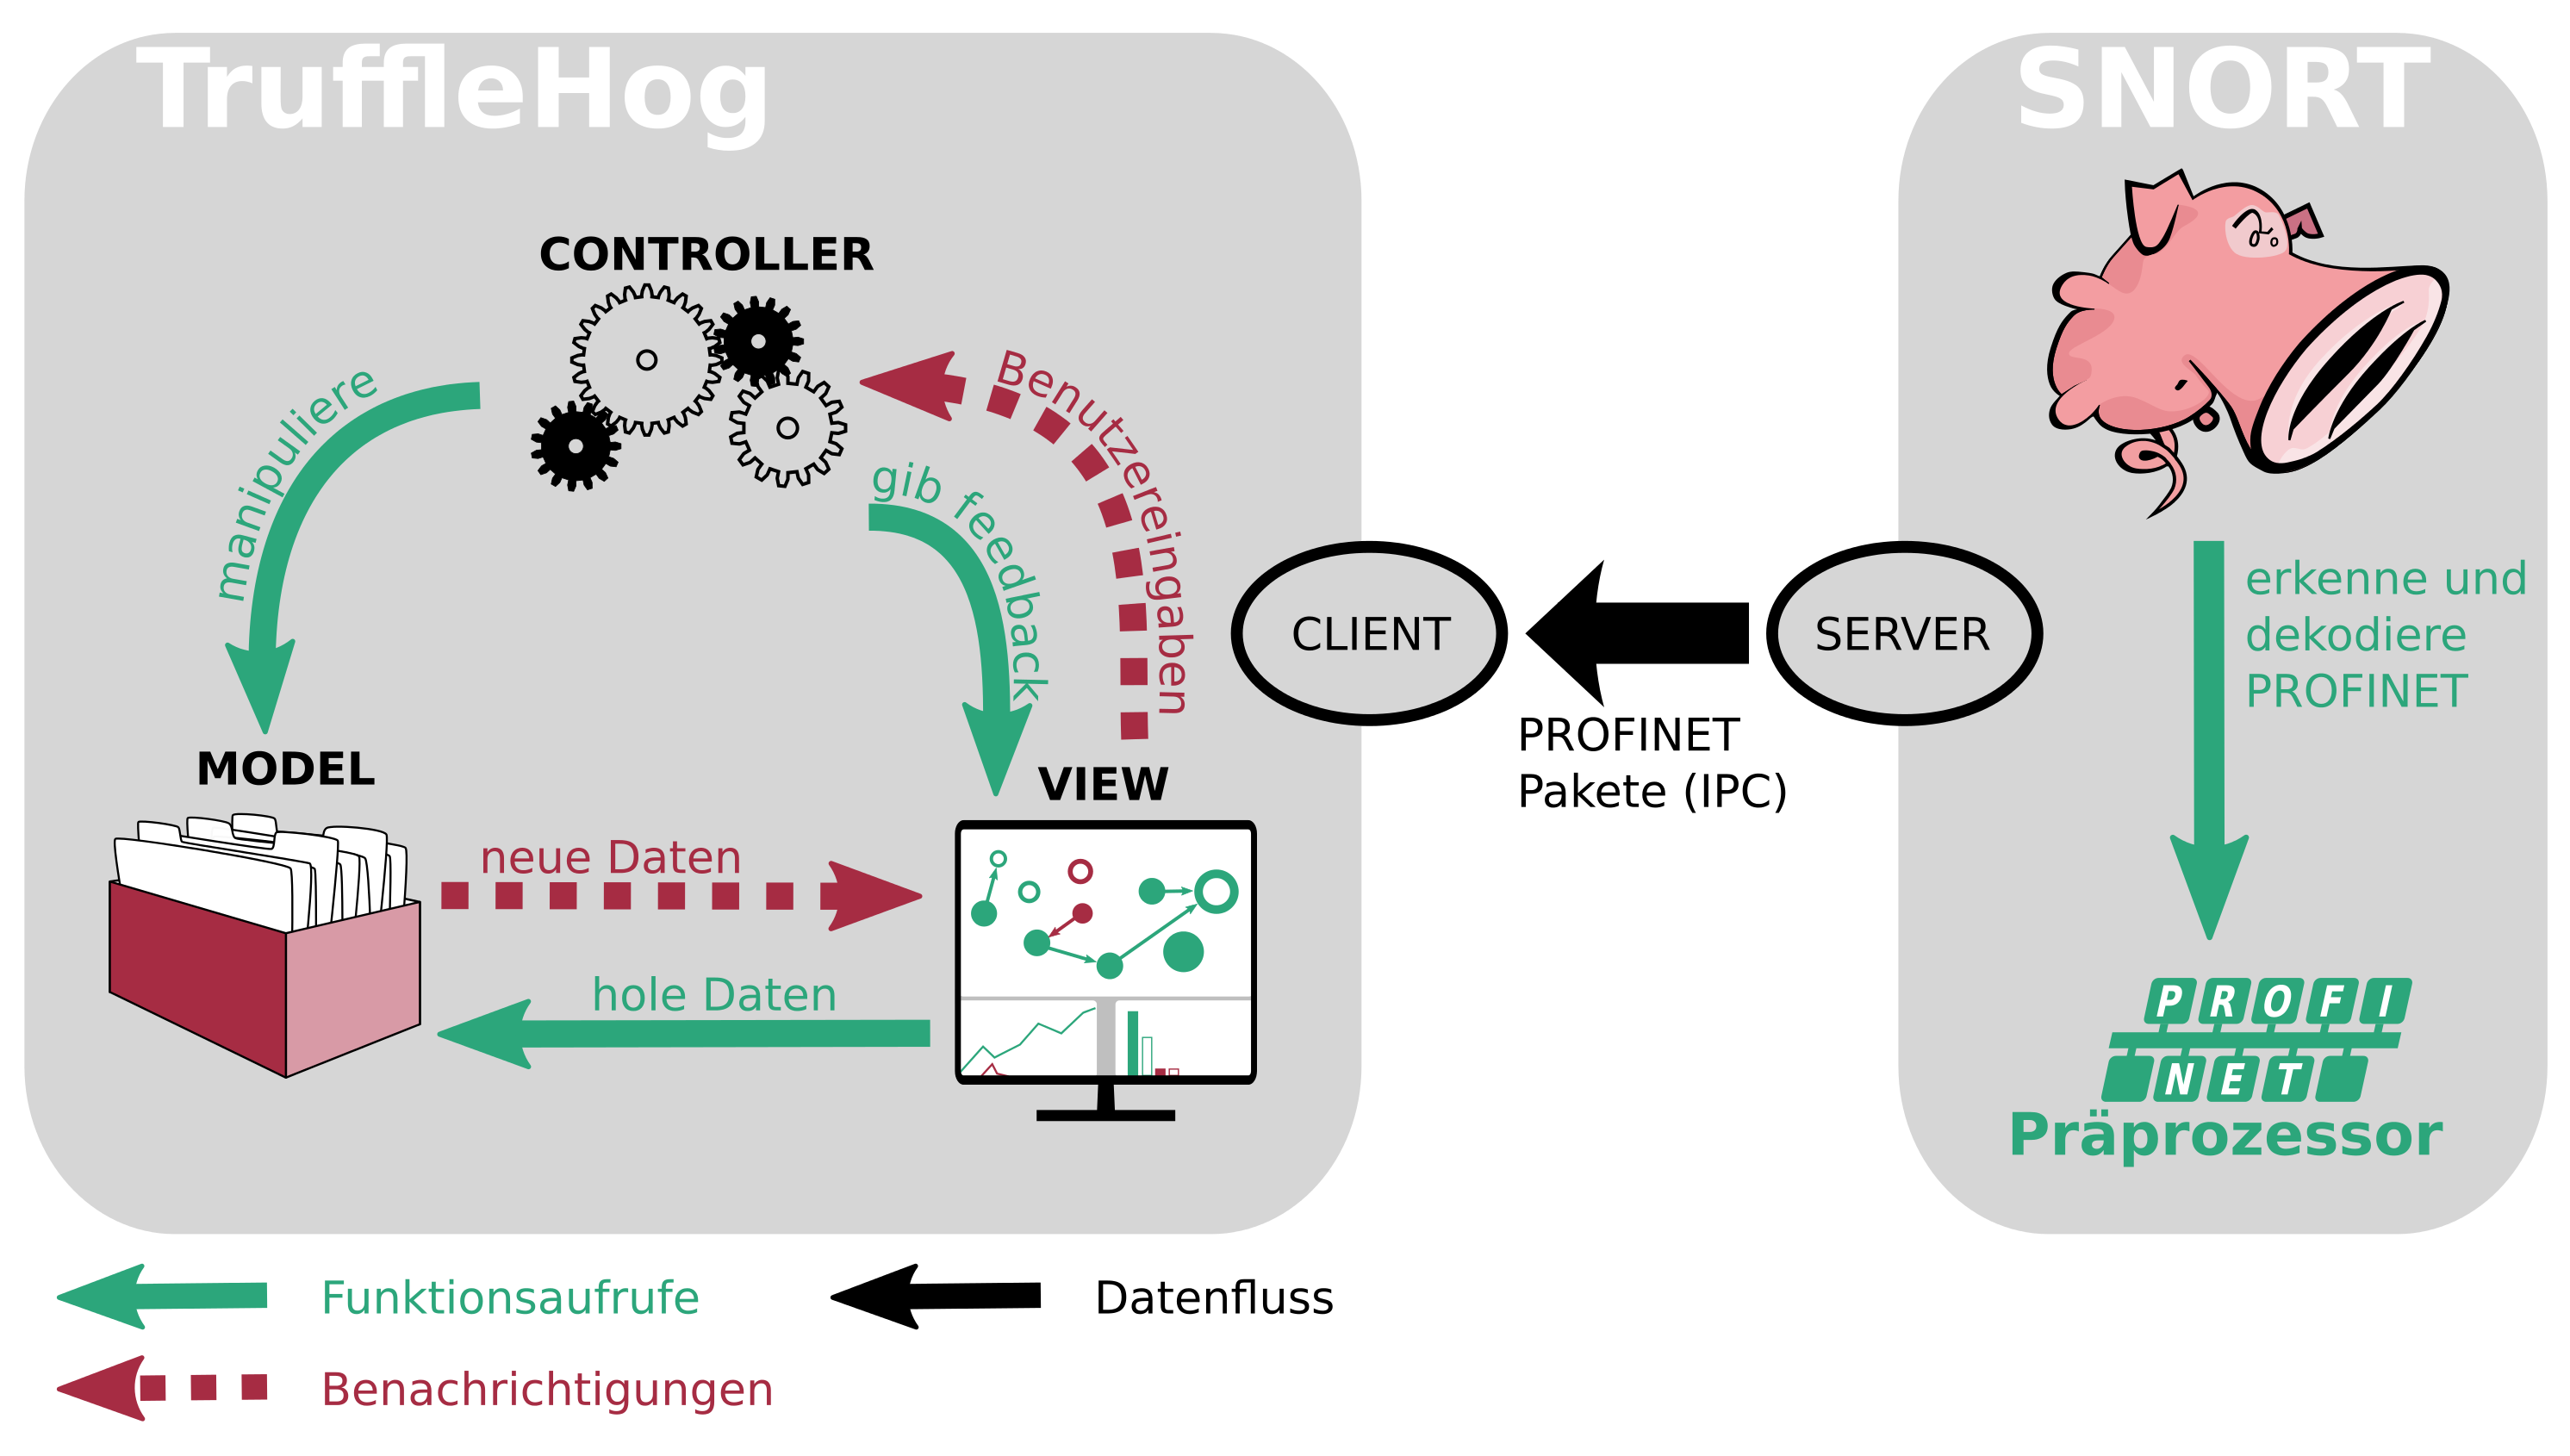
\includegraphics[width=\textwidth]{../diagramimages/praesentationsmodel.png}
  \caption[\gls{mvc}]{\gls{mvc}}
  \medskip
  Grobe Struktur aus der Pflichtenheft-Präsentation
\end{figure} 